\section{Background}

\begin{figure*}[!htbp] 
    \centering
    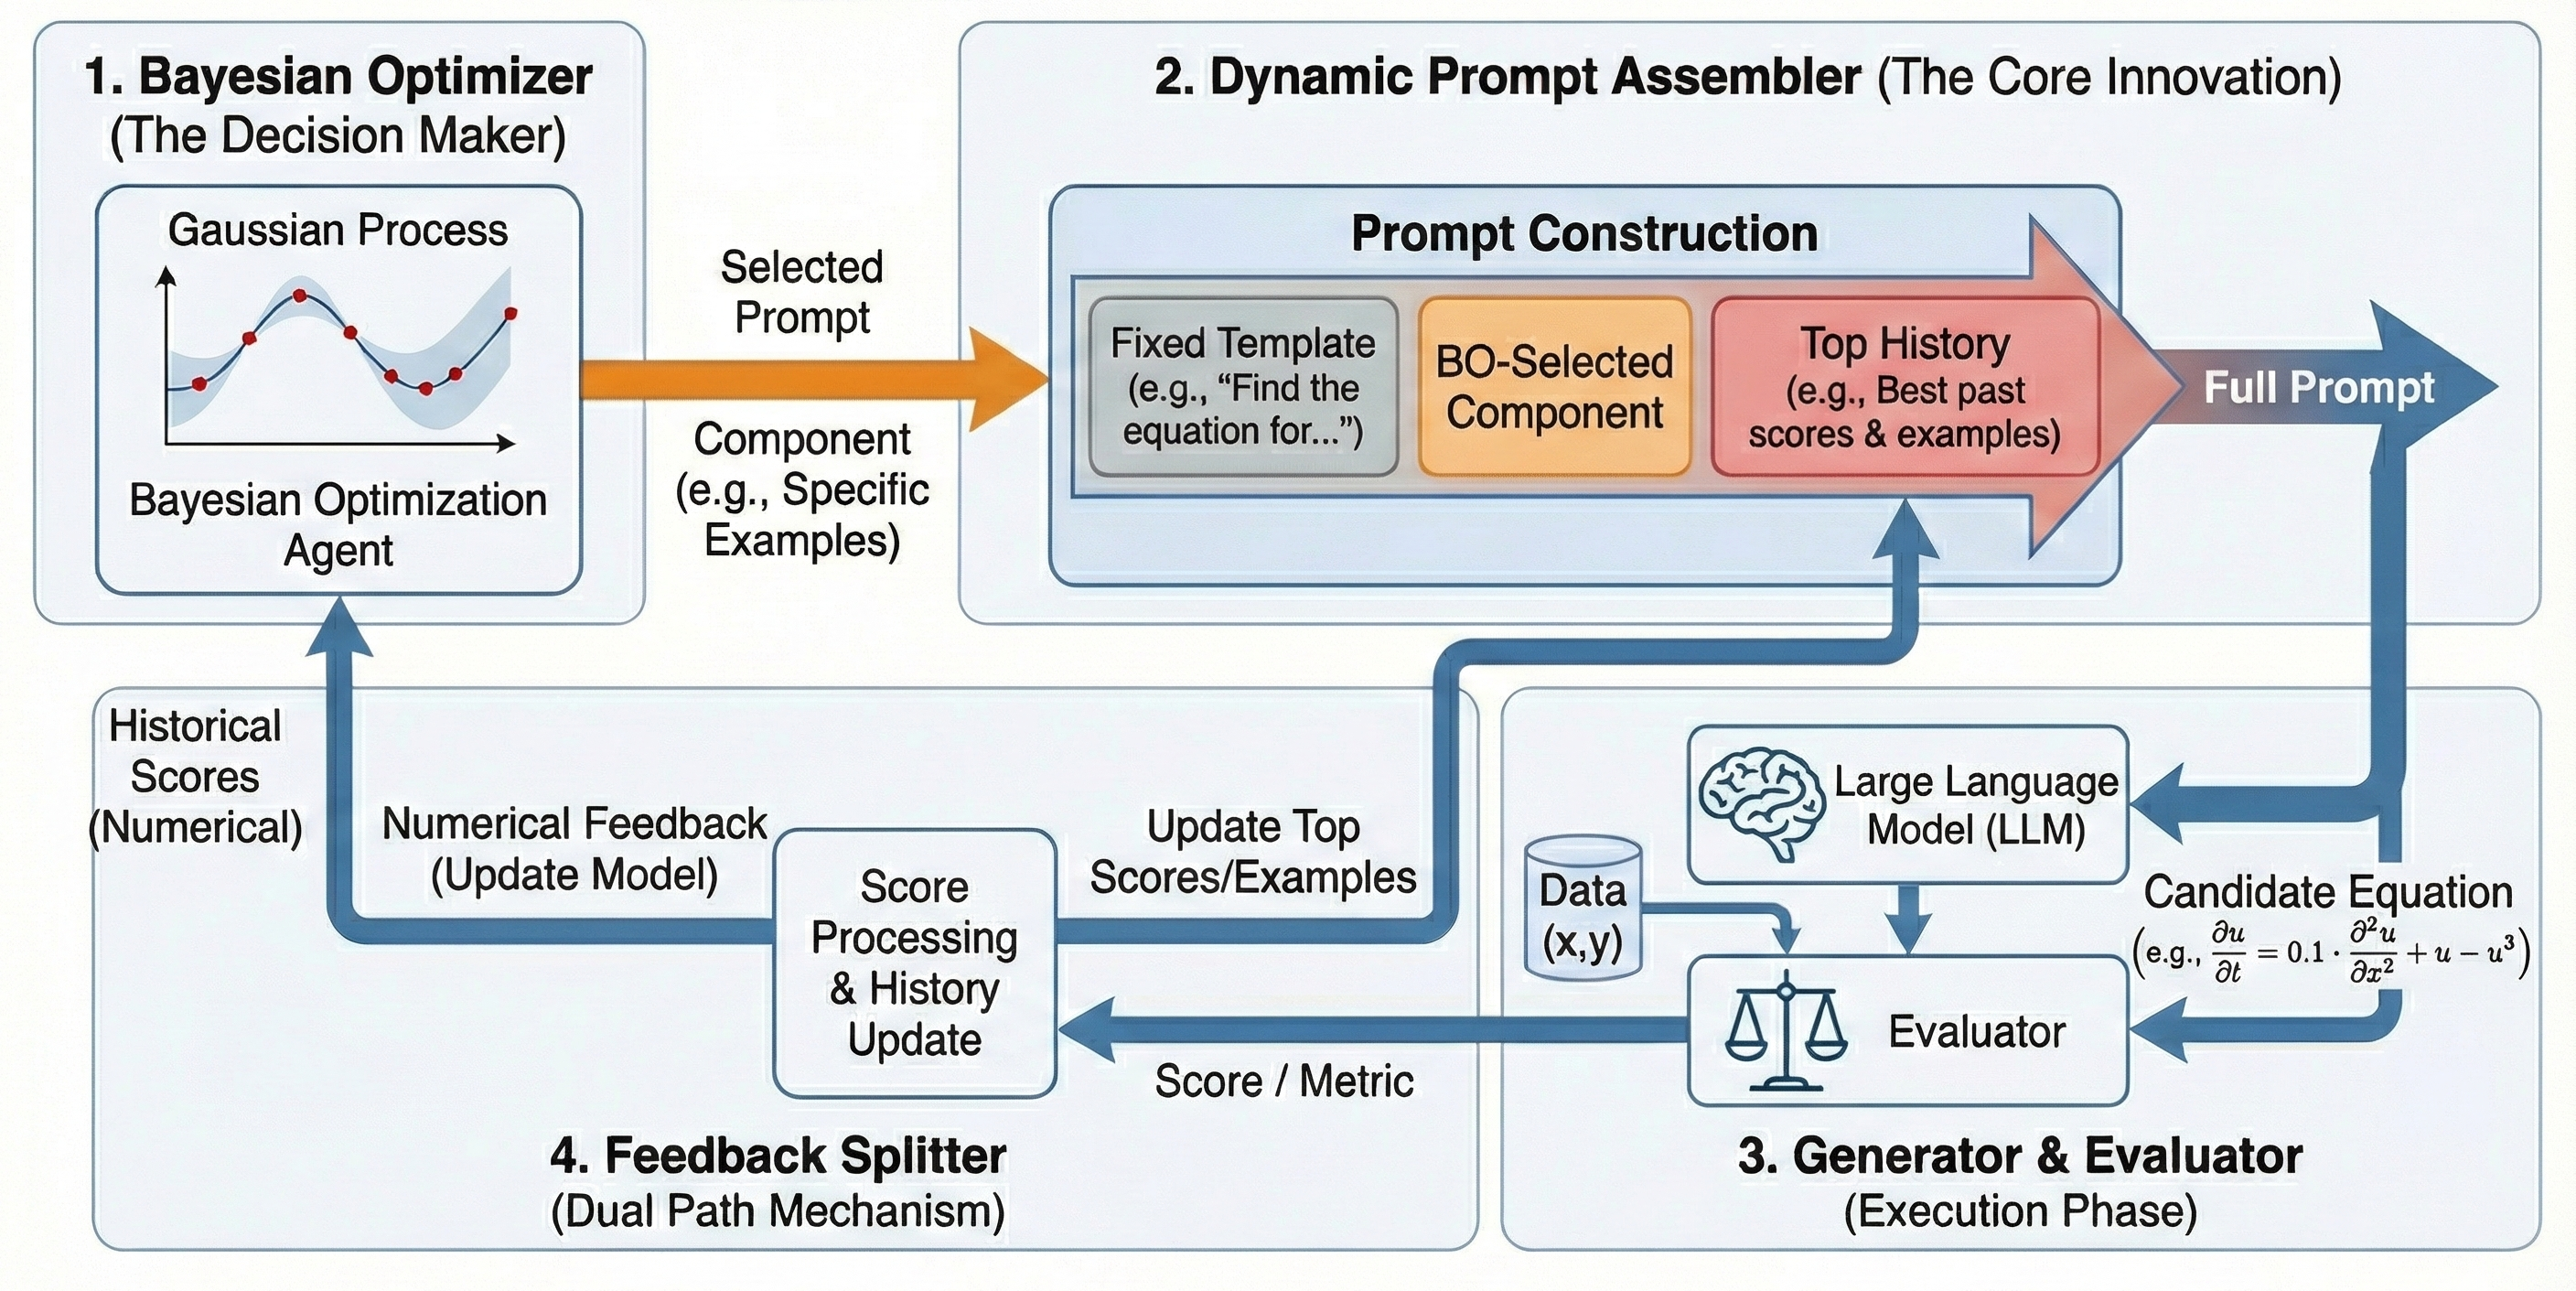
\includegraphics[width=0.9\textwidth]{figs/figure1v1.png} 
    \caption{\small Overview of \textsc{NeuroSym-BO}. A Bayesian Optimizer (1) selects instruction strategies that are assembled into prompts (2) with historical context. The LLM generates candidate equations for evaluation (3), and feedback updates both the history and the optimizer (4), forming a closed-loop system.}
    \label{fig:framework} 

\end{figure*}

\paragraph{PDE Discovery} We consider the task of discovering a governing partial differential equation (PDE) from observational data~\cite{brunton2016sindy,rudy2017pdefind}. Given a spatiotemporal dataset $\mathcal{D} = \{(x_i, t_i, u_i)\}_{i=1}^N$ representing measurements of a physical quantity $u$ at spatial locations $x$ and times $t$, our goal is to recover the symbolic form of the underlying PDE:  $u_t = \mathcal{N}(u, u_x, u_{xx}, \ldots)$ where $\mathcal{N}$ is an unknown nonlinear operator composed of spatial derivatives and algebraic terms. The search space of possible equations is combinatorially large---even with a modest library of operators (addition, multiplication, differentiation), the number of candidate expressions grows exponentially with equation length. This makes exhaustive enumeration intractable and motivates the use of intelligent search strategies.

\paragraph{Bayesian Optimization(BO)} Bayesian Optimization (BO) is a principled framework for optimizing expensive black-box functions \cite{snoek2012practical,jones1998ego,shahriari2016taking}. The key idea is to maintain a probabilistic surrogate model (typically a Gaussian Process)~\citep{rasmussen2006gp} that estimates both the expected value and uncertainty of the objective function at unobserved points. An acquisition function then uses this surrogate to decide which point to evaluate next, balancing the desire to exploit regions with high predicted performance against the need to explore uncertain regions that might contain better solutions.
